\documentclass[tikz,border=5mm]{standalone}
\usetikzlibrary{shapes.geometric, arrows.meta, positioning, fit, backgrounds, calc, shadows}
\begin{document}
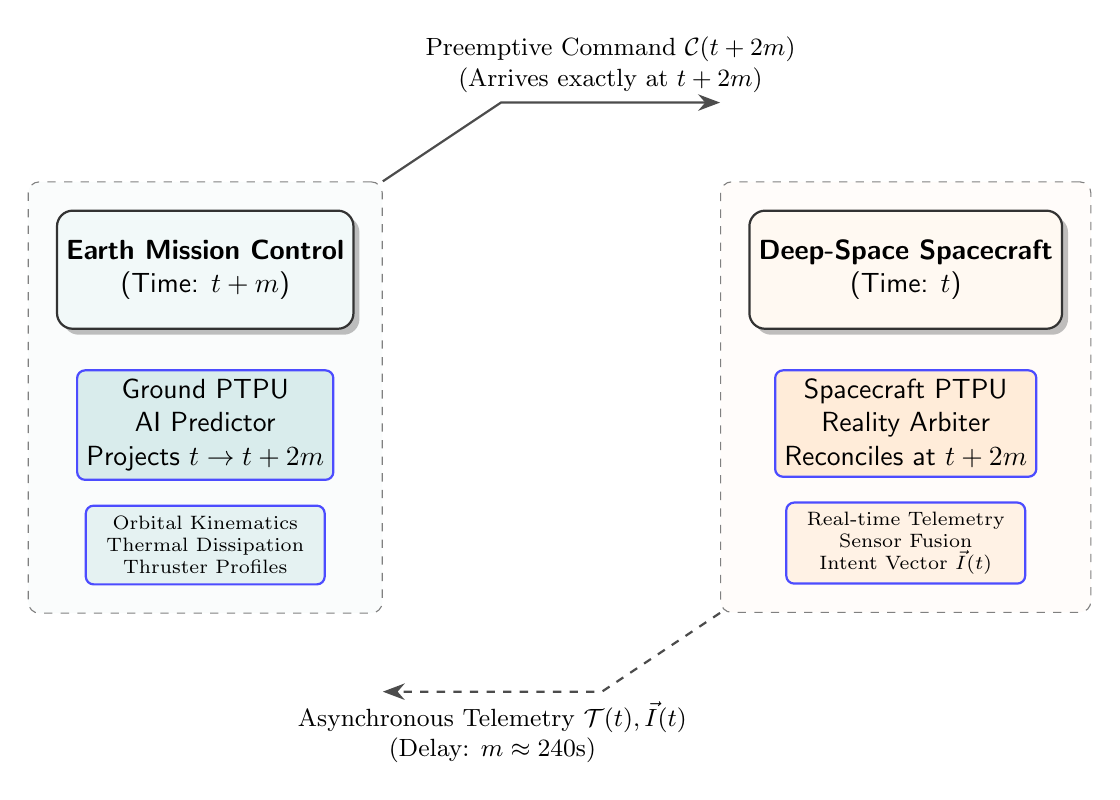
\begin{tikzpicture}[
    font=\sffamily,
    node distance=2cm and 3cm,
    block/.style={rectangle, draw=black!80, fill=blue!5, thick, rounded corners=2mm, minimum width=3.5cm, minimum height=1.5cm, align=center, drop shadow},
    module/.style={rectangle, draw=blue!70, fill=blue!10, thick, rounded corners=1mm, minimum width=3cm, minimum height=1cm, align=center},
    arrow/.style={-{Stealth[scale=1.2]}, thick, draw=black!70},
    dashed_arrow/.style={-{Stealth[scale=1.2]}, dashed, thick, draw=black!70},
    group/.style={rectangle, draw=gray, dashed, inner sep=10pt, rounded corners}
]
% Ground Station
\node[block, fill=teal!5] (ground) {\textbf{Earth Mission Control}\\(Time: $t+m$)};
\node[module, below=0.5cm of ground, fill=teal!15] (earth_ai) {Ground PTPU\\AI Predictor\\Projects $t \to t+2m$};
\node[module, below=0.3cm of earth_ai, fill=teal!10, text width=2.8cm, font=\scriptsize] (earth_models) {Orbital Kinematics\\Thermal Dissipation\\Thruster Profiles};
\begin{scope}[on background layer]
    \node[group, fit=(ground)(earth_ai)(earth_models), fill=teal!2] (earth_group) {};
\end{scope}

% Spacecraft
\node[block, fill=orange!5, right=5cm of ground] (spacecraft) {\textbf{Deep-Space Spacecraft}\\(Time: $t$)};
\node[module, below=0.5cm of spacecraft, fill=orange!15] (cabin_ai) {Spacecraft PTPU\\Reality Arbiter\\Reconciles at $t+2m$};
\node[module, below=0.3cm of cabin_ai, fill=orange!10, text width=2.8cm, font=\scriptsize] (cabin_sensors) {Real-time Telemetry\\Sensor Fusion\\Intent Vector $\vec{I}(t)$};
\begin{scope}[on background layer]
    \node[group, fit=(spacecraft)(cabin_ai)(cabin_sensors), fill=orange!2] (spacecraft_group) {};
\end{scope}

% Comm links
\draw[dashed_arrow] (spacecraft_group.south west) -- ++(-1.5,-1) coordinate(c1) -- node[below, font=\small, align=center] {Asynchronous Telemetry $\mathcal{T}(t), \vec{I}(t)$\\(Delay: $m \approx 240$s)} (earth_group.south east |- c1);

\draw[arrow] (earth_group.north east) -- ++(1.5,1) coordinate(c2) -- node[above, font=\small, align=center] {Preemptive Command $\mathcal{C}(t+2m)$\\(Arrives exactly at $t+2m$)} (spacecraft_group.north west |- c2);

\end{tikzpicture}
\end{document}
